\documentclass[12pt, a4paper]{article}

\usepackage[hmargin=2.5cm, vmargin=2cm]{geometry}
\usepackage{amsthm, amssymb, mathtools, yhmath, graphicx}
\usepackage{fontspec, type1cm, titlesec, titling, fancyhdr, tabularx}
\usepackage{color, unicode-math, float, siunitx}
\usepackage[siunitx]{circuitikz}

\usepackage[CheckSingle, CJKmath]{xeCJK}
\usepackage{CJKulem}
\usepackage{enumitem}
%\setCJKmainfont[BoldFont=cwTex Q Hei]{cwTex Q Ming}
%\setCJKsansfont[BoldFont=cwTex Q Hei]{cwTex Q Ming}
%\setCJKmonofont[BoldFont=cwTex Q Hei]{cwTex Q Ming}
\setCJKmainfont[BoldFont=cwTeX Q Hei]{cwTeX Q Ming}

\def\normalsize{\fontsize{12}{18}\selectfont}
\def\large{\fontsize{14}{21}\selectfont}
\def\Large{\fontsize{16}{24}\selectfont}
\def\LARGE{\fontsize{18}{27}\selectfont}
\def\huge{\fontsize{20}{30}\selectfont}

%\titleformat{\section}{\bf\Large}{\arabic{section}}{24pt}{}
%\titleformat{\subsection}{\large}{\arabic{subsection}.}{12pt}{}
%\titlespacing*{\subsection}{0pt}{0pt}{1.5ex}

\parindent=24pt

\DeclarePairedDelimiter{\abs}{\lvert}{\rvert}
\DeclarePairedDelimiter{\norm}{\lVert}{\rVert}
\DeclarePairedDelimiter{\inpd}{\langle}{\rangle}
\DeclarePairedDelimiter{\ceil}{\lceil}{\rceil}
\DeclarePairedDelimiter{\floor}{\lfloor}{\rfloor}

\newcommand{\samp}{\si{\ampere}}
\newcommand{\smia}{\si{\milli\ampere}}
\newcommand{\svol}{\si{\volt}}
\newcommand{\sohm}{\si{\ohm}}
\newcommand{\skom}{\si{\kilo\ohm}}
\newcommand{\sdb}{\si{\decibel}}
\newcommand{\img}{\mathrm{i}}

\begin{document}

\section{2.27}
The circuit in Fig. P2.27 can be can be consider to be an extension of the circuit in Fig. 2.8

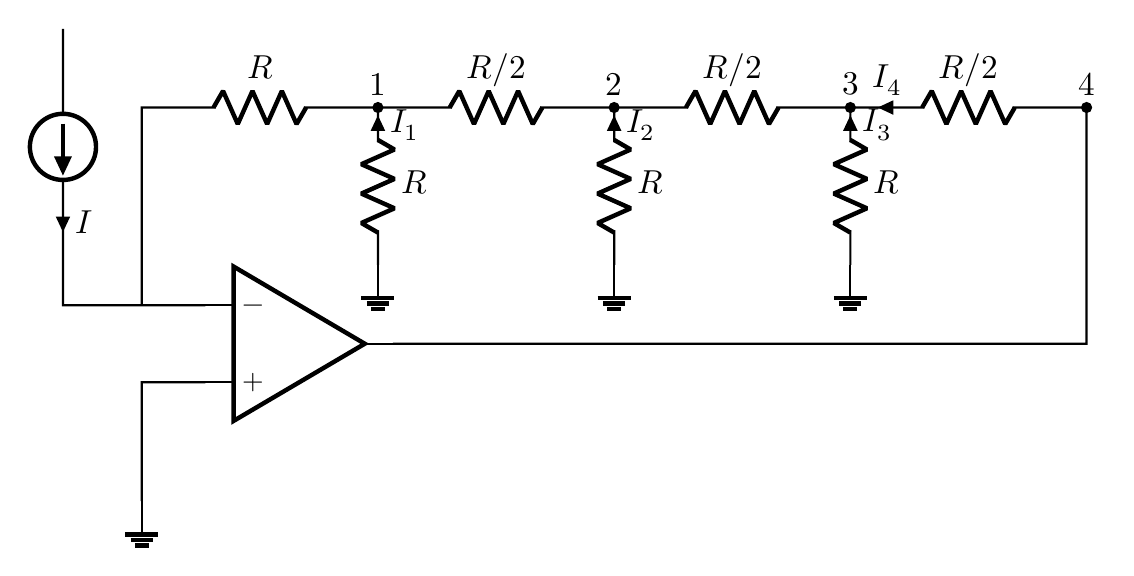
\begin{tikzpicture}[american voltages, american currents]
	\draw[color=black, thick]
  (0, 6) to [I=$I$] (0, 3) 
  %(0, 3) to [short] (3, 3)
  (3, 2) node[op amp](op) {}
  (op.-) -| (0, 3)
  (op.-) -| (1, 5) to[R, l=$R$, -*] (4, 5) to[R, l=$R/2$ ,-*] (7, 5) to[R, l=$R/2$, -*] (10, 5) to[R, l=$R/2$, i<=$I_4$, -*] (13, 5)
  (op.out) -| (13, 5)
  (4, 5) to [R, l=$R$, i<=$I_1$] (4, 3) node[ground]{}
  (7, 5) to [R, l=$R$, i<=$I_2$] (7, 3) node[ground]{}
  (10, 5) to [R, l=$R$, i<=$I_3$] (10, 3) node[ground]{}
  (op.+) -| (1, 0) node[ground]{}
  (4, 5) node[above]{$1$}
  (7, 5) node[above]{$2$}
  (10, 5) node[above]{$3$}
  (13, 5) node[above]{$4$}
	;
\end{tikzpicture}

\begin{enumerate}[label=(\alph*)]
  \item Find the resistance looking into node 1, 2, 3, 4.\\
    Ans: 
    \begin{align*}
      R_1 &= R\\
      R_2 &= (R || R) + R / 2 = R\\
      R_3 &= (R || R) + R / 2 = R\\
      R_4 &= (R || R) + R / 2 = R\\
    \end{align*}
  \item Find the currents $I_1, I_2, I_3, I_4$, in terms of $I$
    Ans:
    \begin{align*}
      I_1 &= IR / R = I\\
      I_2 &= ((I+I_1) (R/2) + IR) / R= 2I\\
      I_3 &= (4IR/2 + 2IR)/R = 4I \\
      I_4 &= (8IR/2 + 4IR)/R = 8I 
    \end{align*}
  \item Find the voltages at node 1, 2, 3, 4.\\
    Ans:
    \begin{align*}
      V_1 &= IR               \\
      V_2 &= V_1 + 2IR/2 = 2IR\\
      V_3 &= V_2 + 4IR/2 = 4IR\\
      V_4 &= V_3 + 8IR/2 = 8IR
    \end{align*}
\end{enumerate}

\section{2.28}
The circuit below utilizes an ideal op amp.\\
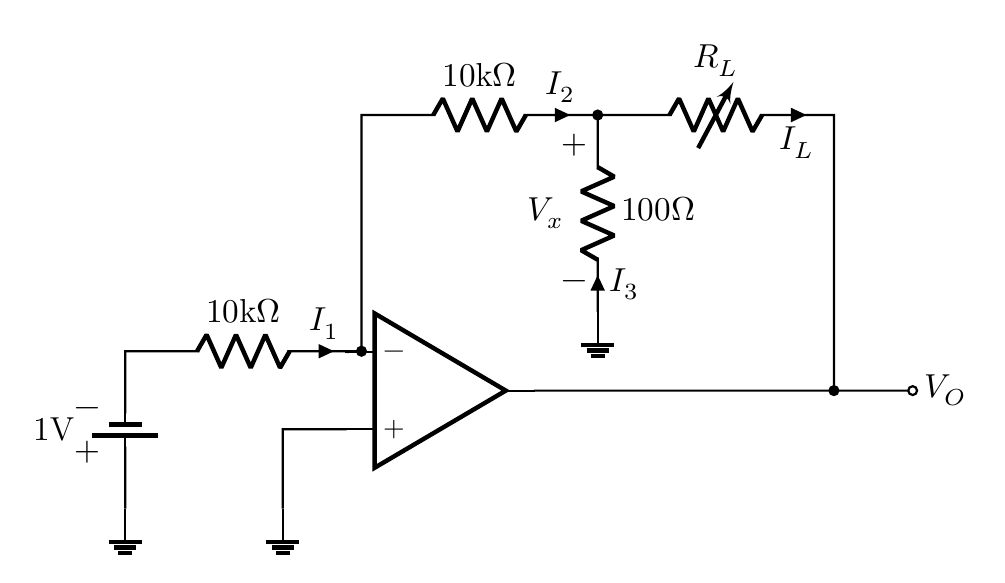
\begin{tikzpicture}[american voltages, american currents]
	\draw[color=black, thick]
  (0, 0) node[ground]{} to [battery1=$1\si{\volt}$] (0, 2) to [R, l=$10\si{\kilo\ohm}$, i>=$I_1$, -*] (3, 2) -- (3, 5) to [R, l=$10\si{\kilo\ohm}$, i>=$I_2$, -*] (6, 5)
  (6, 5) to [vR, l=$R_L$, i_>=$I_L$] (9, 5) -| (9, 1.5)
  (4, 1.5) node[op amp](op) {}
  (op.-) to [short] (3, 2)
  (2, 0) node[ground]{} |- (op.+)
  (op.out) to [short, -*] (9, 1.5) to [short, -o] (10, 1.5) node[right]{$V_O$}
  (6, 5) to [R, l=$100\si{\ohm}$, v=$V_x$, i^<=$I_3$] (6, 2.5) node[ground]{}
	;
\end{tikzpicture}
\begin{enumerate}[label=(\alph*)]
  \item Find $I_1, I_2, I_3, V_x$\\
    Ans: 
    \begin{align*}
      I_1 &= 1\si{\volt} / 10\si{\kilo\ohm} = 0.1\si{\milli\ampere}\\
      I_2 &= I_1 = 0.1\si{\milli\ampere}\\
      V_x &= 0 - (0.1\si{\milli\ampere})(10\si{\kilo\ohm}) = -1 \si{\volt}\\
      I_3 &= 1 / 100\si{\ohm} = 10\si{\milli\ampere}
    \end{align*}
  \item If $V_O$ is not to be lower than $-13\si{\volt}$, find the maximum allowed value of $R_L$\\
    Ans: 
    \begin{align*}
      V_O &= V_x + R_L I_L = V_x + R_L (I_2 + I_3)\\
          &= - 1\si{\volt} - (10.1 \smia) R_L
    \end{align*}
    so
    \[
      R_L \leq 12\svol / 10.1 \smia \approx 1.19
    \]
  \item If $R_L$ is varied in the range $100 \sohm$ to $1 \si{\kilo\ohm}$, what is the corresponding change in $I_L$ and in $V_O$?
    $I_L$ would not change\\
    \[
      V_O \rvert_{R_L = 100 \sohm} = 2.02 \svol, V_O \rvert_{R_L = 1\skom} = 11.2\svol
    \]
\end{enumerate}


\section{2.37}
Figure P2.37 shows a circuit for a digital-to-analog converter.
Show that $v_O$ is given by
\[
  v_O = - \frac{R_f}{16} \sum_{i=0}^{3} 2^i a_i
\]

\section{2.51}
Figure shows a circuit that provides an output voltage $v_o$ whose value can be varied by turning the wiper of the 100\skom potentiometer. Find the range over which $v_o$ can be varied. If the potentiometer is a "20-turn" device, find the change in $v_o$ corresponding to each turn of the pot.

\section{2.63}
For an instrumentation amplifier of the type shown in Fig 2.20(b), a designer proposes to make $R_2 = R_3 = R_4 = 100\skom$ and $2R_1 = 10\skom$. For ideal components, what difference-mode gain, common-mode gain, and CMRR result? Reevaluate the worst-case values for these for the situation in which all resistors are specified as $\pm 1\%$ units. Repeat the latter analysis for the case in which $2R_1$ is reduced to $1 \skom$. What do you conclude about the importance of the relative difference gains of the first and second stages?

\section{2.65}
The circuit shown in Fig is intended to supply a voltage to floating loads (those for which both terminals are ungrounded) while making possible use of available power supply.

\section{2.66}
The two circuits in Fig are intended to function as voltage-to-current converters; that is, they supply the load impedance $Z_L$ with a current proportional to $v_I$ and independent of the value of $Z_L$. Show that this is indeed the case, and find for each circuit $i_o$ as a function of $v_I$. Comment on the differences between the two circuits.

\section{2.69}
An op-amp-based inverting integrator is measured at $1 \si{\kilo\hertz}$ to have a voltage gain of $-100\si{V/V}$. At what frequency is its gain reduced to $-1 \si{V/V}$? What is the integrator time constant?

\section{2.79}
Derive the transfer function of the circuit in Fig and show that it can be written in the form
\[
  \frac{V_o}{V_i} = \frac{-R_2/R_1}{\left(1+(\omega_1/(\img\omega))\right)\left(1+(\omega/(\img\omega_2))\right)}
\]


\section{2.100}
A designer, wanting to achieve a stable gain of $100 \si{V/V}$ at $5 \si{\mega\hertz}$, considers her choice of amplifier topologies. What unity-gain frequency would a single operational amplifier require to satisfy her need? Unfortunately, the best available amplifier has an $f_t$ of $40 \si{\mega\hertz}$. How many such stages would she need to achieve her goal? What is the $3\sdb$ frequency of each stage she can use? What is the overall $3\sdb$ frequency?

\section{2.102}
Consider an inverting summer with two inputs $V_1$ and $V_2$ and with $V_O = -(V_1 + V_2)$. Find the $3 \sdb$ frequency of each of the gain functions $V_o / V_1$ and $V_o / V_2$ in terms of the op amp $f_1$.

\section{2.104}
An op amp having a slew rate of $20 \si{V/\micro s}$ is to be used in the unity-gain follower configuration, with input pulses that rise from $0$ to $3\svol$. What is the shortest pulse that can be used while ensuring full-amplitude output? For such a pulse, describe the outputing resulting.


\end{document}

